\newpage
\section{What is an Isometry?}

In this activity, we are going to explore the geometry of isometries.
\[
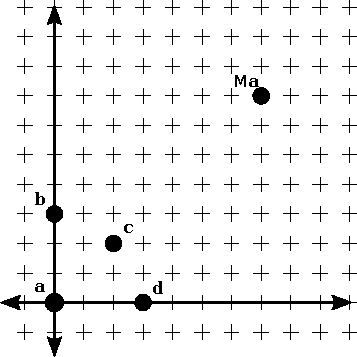
\includegraphics{../graphics/planeIso.pdf}
\]

\begin{prob}
Remind me, gentle reader, what is the definition of an isometry?
\end{prob}

\begin{prob}
Suppose that some isometry $\mat{M}$ moves point $\vec{a}$ to
$\mat{M}\vec{a}$. Carefully draw all possible locations for
$\mat{M}\vec{b}$.
\end{prob}

\begin{prob}
Now suppose that the same isometry $\mat{M}$ moves point $\vec{c}$ to
$\mat{M}\vec{c} = (5,5)$. Indicate all possible locations for
$\mat{M}\vec{b}$.
\end{prob}

\begin{prob}
Now suppose that the same isometry $\mat{M}$ moves point $\vec{d}$ to
$\mat{M}\vec{d} = (7,4)$. Indicate all possible locations for
$\mat{M}\vec{b}$.
\end{prob}



\begin{prob}
Finally, consider point $\vec{e} = (1,5)$. Where is $\mat{M}\vec{e}$?
\end{prob}

